\documentclass[aspectratio=169]{beamer}
\usetheme{Madrid}
\usecolortheme{default}

\usepackage{booktabs}
\usepackage{graphicx}
\usepackage{array}

\title[Annealed Router Labels]{Annealed Weak Router Supervision}
\subtitle{Branch Specialization Phase 3 Toy Checkpoint}
\author{Branch specialization research project}
\date{2026-05-22}

\begin{document}

\begin{frame}
  \titlepage
  \vspace{-0.5em}
  \small
  Checkpoint reason: the annealed-label experiment changes the next research
  step from broad regularizer sweeps to training-time trajectory measurement.
\end{frame}

\begin{frame}{Current Question}
  \textbf{Question.} Does role-informative routing pressure only need to break
  symmetry early, or must it remain active through most of training for
  branch-level functional modularity to persist?

  \vspace{1em}
  \textbf{Setting.} The conflict task makes the same query token require two
  incompatible role rules:
  \begin{itemize}
    \item local role: predecessor lookup, $y_i \rightarrow y_{i-1}$;
    \item induction role: successor lookup, $y_i \rightarrow y_{i+1}$.
  \end{itemize}

  \vspace{0.5em}
  Earlier checkpoints showed that unlabeled routing pressure, branch
  bottlenecks, and conflict alone did not produce role-aligned causal branch
  modularity, while weak role labels did.
\end{frame}

\begin{frame}{Experimental Schedule}
  \begin{itemize}
    \item Model: \texttt{weak\_token\_router}
    \item Task: \texttt{bidirectional\_lookup}
    \item Branch head dimension: 64
    \item Training: 1600 steps, 5 seeds, equal local/induction loss weight
    \item Weak router-label loss: weight 0.05 while active
  \end{itemize}

  \vspace{0.8em}
  \begin{center}
  \begin{tabular}{lrrrrrrr}
    \toprule
    Label end step & 50 & 100 & 200 & 400 & 800 & 1200 & always \\
    Fraction of training & .03 & .06 & .12 & .25 & .50 & .75 & 1.00 \\
    \bottomrule
  \end{tabular}
  \end{center}

  \vspace{0.8em}
  The new flag is \texttt{--router-supervision-end-step N}; weak labels are
  active only for optimization steps $<N$.
\end{frame}

\begin{frame}{Metric Glossary}
  \begin{description}
    \item[Same top branch] Fraction of seeds where local and induction both have
    the same most-important branch under causal branch ablation.
    \item[Routed role match] Fraction of seeds where local maps to branch 0 and
    induction maps to branch 1 under causal branch ablation.
    \item[Branch distance] Average distance between the causal branch-use
    distributions for local and induction roles. Larger means stronger
    separation.
    \item[Gate routed match] Whether router probabilities put the two roles on
    the intended branches. This is not enough by itself; the branch computation
    must also be causally separable.
  \end{description}
\end{frame}

\begin{frame}{Main Evidence}
  \begin{center}
    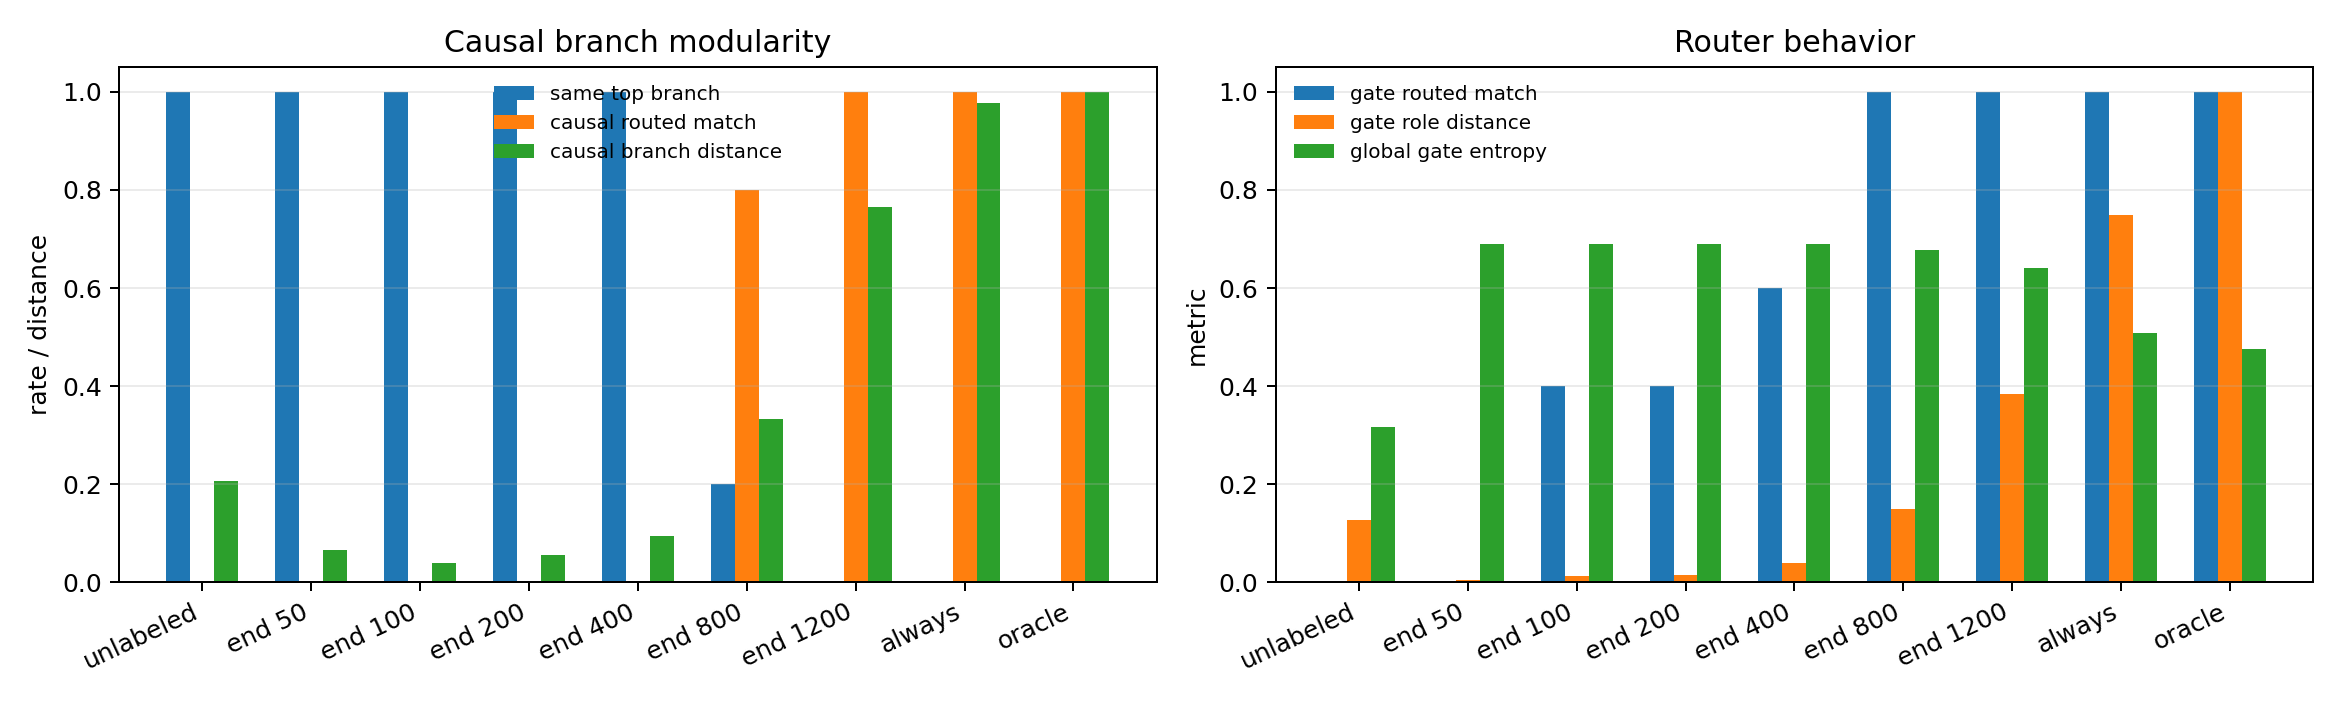
\includegraphics[width=0.96\linewidth]{figures/annealed_router_comparison.png}
  \end{center}

  \small
  Left: causal branch modularity metrics. Right: router probability metrics.
  The discontinuity between end 400 and end 800 is the key empirical threshold
  in this toy setup.
\end{frame}

\begin{frame}{Results Table}
  \small
  \begin{center}
  \begin{tabular}{lrrrr}
    \toprule
    Condition & Label fraction & Same top & Routed match & Branch dist. \\
    \midrule
    unlabeled entropy+balance & 0.00 & 1.00 & 0.00 & 0.2069 \\
    end 50 & 0.03 & 1.00 & 0.00 & 0.0670 \\
    end 400 & 0.25 & 1.00 & 0.00 & 0.0945 \\
    end 800 & 0.50 & 0.20 & 0.80 & 0.3337 \\
    end 1200 & 0.75 & 0.00 & 1.00 & 0.7652 \\
    always label 0.05 & 1.00 & 0.00 & 1.00 & 0.9773 \\
    oracle route & -- & 0.00 & 1.00 & 1.0000 \\
    \bottomrule
  \end{tabular}
  \end{center}

  \vspace{0.8em}
  \textbf{Readout.} Brief early labels solve the task but do not preserve causal
  role separation. Labels through 75\% of training preserve the top-branch split
  after removal, but with weaker separation than always-on labels.
\end{frame}

\begin{frame}{Interpretation}
  \textbf{Supported by this run}
  \begin{itemize}
    \item Role-informative pressure does not need to remain active until the
    final step for a top-branch role split to persist.
    \item In this setup, it must last through a large fraction of training.
    \item Continuous role pressure gives stronger causal separation than late
    removal.
  \end{itemize}

  \vspace{0.8em}
  \textbf{Not supported}
  \begin{itemize}
    \item Brief role labels as a small early symmetry-breaking nudge.
    \item The stronger claim that structural branches plus task pressure alone
    reliably become functional branch modularity.
  \end{itemize}
\end{frame}

\begin{frame}{Project-Level Update}
  \textbf{Best current toy conclusion.}

  \vspace{0.5em}
  Structural branch design is a substrate. In these toy runs, it did not by
  itself produce functional branch modularity, even with conflict, bottlenecks,
  entropy regularization, or load balancing.

  \vspace{0.8em}
  The reliable ingredient observed so far is role-informative routing pressure.
  That pressure can be removed late with partial persistence, but short early
  exposure is not enough.

  \vspace{1em}
  This reframes the next question:
  \begin{center}
  \textit{What training signal makes structural modularity become functional
  modularity, and when must that signal be present?}
  \end{center}
\end{frame}

\begin{frame}{Decision And Next Experiment}
  \textbf{Decision.} Stop broad sweeps of generic unlabeled router regularizers
  for this toy branch.

  \vspace{0.8em}
  \textbf{Next decisive experiment.}
  Add training-time checkpointing and evaluate gate and causal branch separation
  at intermediate steps:
  \begin{itemize}
    \item before label removal;
    \item immediately after label removal;
    \item late in training after task loss has acted without labels.
  \end{itemize}

  \vspace{0.8em}
  Priority schedules: end 400, end 800, end 1200, always-on, and unlabeled
  entropy+balance.
\end{frame}

\begin{frame}{Provenance}
  \small
  \textbf{Source files}
  \begin{itemize}
    \item \texttt{scripts/toy\_branch\_isolation\_intervention.py}
    \item \texttt{scripts/analyze\_annealed\_router\_experiment.py}
    \item \texttt{doc/phase3\_toy\_annealed\_router.md}
  \end{itemize}

  \vspace{0.5em}
  \textbf{Copied data in this deck folder}
  \begin{itemize}
    \item \texttt{data/annealed\_summary.csv}
    \item \texttt{data/annealed\_with\_references.csv}
    \item \texttt{figures/annealed\_router\_comparison.png}
  \end{itemize}

  \vspace{0.5em}
  \textbf{Rebuild}
  \begin{itemize}
    \item \texttt{python3 -u scripts/analyze\_annealed\_router\_experiment.py}
    \item \texttt{python3 .../compile\_latex\_deck.py presentations/2026-05-22-1709-annealed-router/annealed\_router\_checkpoint.tex}
  \end{itemize}
\end{frame}

\end{document}
